\section{Evaluation}
\label{SEC:evaluation}

CrashSimulator was designed
as a way to reduce the considerable effort
required of developers
in implementing and maintaining applications.
Therefore,
we needed to prove its effectiveness in ``the wild.''
To this end,
we carried out two rounds of
evaluation for CrashSimulator.
We started by exposing
a series of real-world applications
to a library of collected anomalies in a laboratory environment.
These tests,
conducted by the research team,
were followed by a user study
in which undergraduate and graduate computer science students
got a chance to use CrashSimulator
to identify new environmental bugs
in tests on applications of their choosing.
We used the results from both these efforts
to answer the following questions:

\begin{enumerate}

\item{Is CrashSimulator able to identify bugs in real world applications?
    (Subsection~\ref{sec-env-bugs})}

\item{What sorts of errors does CrashSimulator make?
    (Subsection~\ref{sec-sorts-errors})}

\item{Can CrashSimulator
      execute tests efficiently? (Subsection~\ref{sec-perf})}

\end{enumerate}

\subsection{Is CrashSimulator able to identify bugs in real world
applications?}
\label{sec-env-bugs}

The most crucial question to ask about the SEA technique and the tool we implemented from it is can we
identify bugs
caused by different types of problematic environmental features.
We have already established
that
unusual filesystem and network situations can cause an application to fail,
so we configured the tool to look
for bugs that could be triggered in this manner.
We found the specific anomalies used for this evaluation
by examining public bug trackers,
the source code of major portable applications, and the capabilities of
tools like NetCheck~\cite{Zhuang_NSDI_2014}
and CheckAPI~\cite{rasley2015detecting}.
As we wanted to test
the most commonly used applications,
our selections were made
from among those deemed ``popular''
by Debian's Popularity Contest~\cite{DebPopCon},
or those used
by many Linux distributions,
such as ones provided
by the GNU Coreutils project.

\subsubsection{The simplest case - A Filesystem Bug Found With the Null Mutator}
\label{sec-move-bugs}
In our first test we decided to evaluate the tool in its simplest possible
configuration -- employing the {\bf ``null mutator.''}
This mutator takes no action and simulates no anomalous conditions.
It simply allows checkers to evaluate an application's behavior
as it carries out a potentially-buggy operation.
We decided to look at how applications
move files around on the filesystem.
Though, in many cases, this operation can be handled
atomically by the operating system
through the {\tt rename()} system call,
in situations where
the source file and destination file are on different storage devices,
the operation must be performed manually by the application.
This is a process
that even well-tested applications
frequently get wrong~\cite{PHPRenameBug,PythonShutilBug,NodejsCopyBug}.

{\bf Method.}
CrashSimulator was configured
to test each of the applications listed in Table~\ref{table:crossdevice}
to see which might fail to correctly move a file from one disk to another.
The tests were completed using just the Null Mutator and a set of
checkers that model the correct steps involved in moving a file from one
storage device to another.
After examining several libraries and applications,
we found that
{\tt mv} seemed to handle cases that other tools failed to consider.
Therefore, we
used its behavior as a template to create a set of checkers
that evaluate whether or not
the application correctly performs the following
steps.

\begin{itemize}
    \item{{\it Confirm Source Not Replaced During Copy.} An application
        should make an effort to ensure that the file being copied is not replaced between the time it is initially examined and when it is opened for copying.
If these checks are not performed, it
means the application will proceed with its operations,
        making file corruption~\cite{PythonShutilBug}} possible.

    \item{{\it Preserve Extended File Attributes.}
When copying a file,
an application should retrieve extended file attributes from the source
file and, later, apply them to the destination file.  Failure to do so can lead to security problems~\cite{AppleCodeSigning}.}

    \item{{\it Preserve Timestamps.}  It is important to ensure
that time related metadata --
such as creation, modification, and access times  --
are preserved when copying a file, as
incorrect timestamps can impede applications like {\tt make},
        archival programs, and similar software~\cite{NautilusTimestamps,
        SudoTimestamp}.}

    \item{{\it Copy Devices Correctly.}
Files of this variety must be moved
by creating a new device of the same type at the destination,
instead of exhaustively reading and writing its contents.
In our experience, applications that fail to perform this check
can end up completely filling disks, exhausting available memory,
        or blocking forever, which can cause the system to become unresponsive.}

\end{itemize}

 \begin{table}[t]
    \scriptsize{}
    \begin{tabular}{l p{1cm} p{1cm} p{1.2cm} p{1cm}}
    \toprule{}
        Application     & Source Replaced & Preserve Xattrs & Preserve Timestamps & Copying Devices\\
\hline
        {\tt mv}              & Correct             & Correct         & Correct             & Correct\\
        {\tt mmv}             & Correct             & {\bf Sec. Flaw} & {\bf Time Loss} & Correct\\
        {\tt install}         & Correct             & {\bf Sec. Flaw} & {\bf Time Loss} & {\bf Fill Disk} \\
        {\tt perl File::Copy} & Correct             & {\bf Sec. Flaw} & {\bf Time Loss} & {\bf Fill Disk} \\
        {\tt shutils}         & {\bf Corrupt}	& {\bf Sec. Flaw} 	& Correct             & Correct\\
        {\tt rust}             & Correct             & {\bf Sec. Flaw} & {\bf Time Loss} & {\bf Fill Disk} \\
        {\tt boost::copyfile} & {\bf Corrupt}	      & {\bf Sec. Flaw} & {\bf Time Loss} & {\bf Fill Disk} \\
    \bottomrule{}
    \end{tabular}
    \caption{Applications and libraries analyzed to determine whether or not
      they are able to correctly move a file from one device to another.
Incorrect entries are either missing the needed check or were ineffective.}
    \label{table:crossdevice}
\end{table}

{\bf Findings.}
CrashSimulator was able to identify whether an array of popular programs,
including the standard libraries for the programming languages Python,
Perl,
and Rust,
can correctly perform complex
operations in anomalous situations.
As can be seen from the results in Table~\ref{table:crossdevice}, each of the
applications tested fails to perform one or more of the steps required to
successfully complete a cross-device move.  This is an unfortunate situation
because a failure to perform any one of these steps can result in negative
outcomes for the system as a whole.
Further, these results demonstrate that even well-tested applications
can miss one or more of the steps in a complicated operation.

\subsubsection{A More Complex Case - The Unexpected File Types Mutator}
\label{sec-file-type-bugs}

If a more complex mutator is to be employed, then
CrashSimulator will  simulate anomalies during execution
of an application.
This introduces problematic scenarios
so an application's response
can be evaluated.
For an effective test of the
tool's capabilities to find bugs created in this process,
we needed to pick an anomaly
that would arise during a common situation,
such as when a Linux application retrieves
and processes data from a file.
Linux supports
several special file types,
including
directories,
symbolic links,
character devices,
block devices,
sockets, and
First-In-First-Out (FIFO) pipes.
These special files
use the same system calls
as regular files
(such as {\tt read()} and {\tt write()}),
but they behave in very different ways.
For example,
{\tt /dev/urandom} is a character device
that produces an infinite amount
of pseudo-random data
when read.
If an application
that relies on exhaustively reading the full
contents of a file before processing is provided {\tt /dev/urandom}, it
will fill memory or disk space, and could
crash the system~\cite{YumAptEndless}.
Correct execution in these situations
requires that applications
examine the files, so they do not
interact inappropriately with a given file type.

{\bf Method.}
Identifying these bugs involves changing an application's
execution to induce its response to an unexpected file type. For
example, the {\tt sed} application, which modifies the contents of a text
file according to a provided command string, could instead be provided a symbolic
link, a directory, or a character device.  CrashSimulator
accomplishes this by identifying the calls to {\tt stat()}, {\tt fstat()},
or {\tt lstat()} that an application makes to examine the file, and
changing the results to simulate
one of the special file types.  If the application responds to
this injected information, then its likely the special
file will be handled correctly.  On the other hand, if there is no
alteration in the behavior of the application, the condition is not
being handled correctly.

For each application,
CrashSimulator was configured to simulate all of the non-standard file
types.
The values inserted into results of the application's {\tt stat()}-like
system calls are listed
in Table~\ref{table:unexpectedtypes}.
A value of ``Expected Type (ET)'' indicates
that this is the file type the application was expecting,
as it matches what was provided when the application was initially recorded.
A result of ``\tickmark'' indicates that the application
identified it was being provided with an unexpected file type and its
execution diverged, a signal that it was potentially handling the
file type correctly.
A result of ``\xmark'' indicates
that the execution never diverged from the trace being replayed,
and thus failed to recognize the presence of an unusual file type.

{\bf Findings.}
The frequency of failed executions in our results,
which are shown in Table 2,
indicates that many
applications assume they will only be used to process
regular files.  When this assumption does not hold, execution results
can be hard to predict.
In many cases a denial of
service condition occurs in the form of the application ``hanging,'' as it
attempts to incorrectly process the file.
This is typically the result of
an application blocking forever as it waits for a {\tt read()}
call to retrieve non-existent data from an empty FIFO,
or an application attempting
to read in and process an
``infinitely large'' file.
This situation is particularly dangerous as
it can eventually
fill all available memory or disk space~\cite{Cappos_CCS_08}.


\begin{table*}[t]
    \scriptsize{}
    \begin{tabular}{l  l  |  l  l  l  l  l  l  l}
    \toprule{}
        Application       & Condition Tested           & Regular File & Directory & Character Device & Block Device & Named Pipe & Symbolic Link & Socket File (IFSOCK)\\
                          &                            &  (IFREG)     & (IFDIR)   & (IFCHR)          & (IFBLK)      & (IFIFO)    & (IFLNK)       & (IFSOCK)\\
\hline
        {\tt Aspell}      & Dictionary File            & ET        & \xmark     & \tickmark  & \xmark    & \xmark        & \xmark       & \xmark\\
        {\tt Aspell}      & File being checked         & ET        & \xmark     & \tickmark  & \xmark    & \xmark        & \xmark       & \xmark\\
        {\tt gnu-gpg}     & secring.gpg                & ET        & \xmark     & \xmark     & \xmark    & \xmark        & \xmark       & \xmark\\
        {\tt vim}         & File being opened          & ET        & \tickmark  & \tickmark  & \tickmark & \tickmark     & \tickmark    & \xmark\\
        {\tt nano}        & File being opened          & ET        & \tickmark  & \tickmark  & \tickmark & \xmark        & \xmark       & \xmark\\
        {\tt sed}         & File being edited          & ET        & \xmark     & \tickmark  & \xmark    & \xmark        & \xmark       & \xmark\\
        {\tt df}          & /proc                      & \xmark    & ET         & \xmark     & \xmark    & \xmark        & \xmark       & \xmark\\
        {\tt wc}          & File being checked         & ET        & \tickmark  & \tickmark  & \tickmark & \tickmark     & \tickmark    & \tickmark\\
        {\tt du}          & Directory being checked    & \tickmark & ET         & \tickmark  & \tickmark & \tickmark     & \tickmark    & \tickmark\\
        {\tt install}     & File being installed       & ET        & \tickmark  & \xmark     & \xmark    & \xmark        & \tickmark    & \xmark\\
        {\tt fmt}         & File being formatted       & ET        & \xmark     & \tickmark  & \xmark    & \xmark        & \xmark       & \xmark\\
        {\tt od}          & File being dumped          & ET        & \tickmark  & \tickmark  & \xmark    & \xmark        & \xmark       & \xmark\\
        {\tt ptx}         & File being read            & ET        & \tickmark  & \tickmark  & \tickmark & \tickmark     & \tickmark    & \tickmark\\
        {\tt comm}        & Second file being compared & ET        & \tickmark  & \tickmark  & \xmark    & \xmark        & \xmark       & \xmark\\
        {\tt pr}          & File being read            & ET        & \tickmark  & \xmark     & \xmark    & \xmark        & \xmark       & \xmark\\
\hline
        \multicolumn{9}{l}{\scriptsize{\tickmark  $=$ CrashSimulator
        predicts application will recognize anomaly}}\\
        \multicolumn{9}{l}{\scriptsize{\xmark  $=$ CrashSimulator predicts
        application will fail to recognize anomaly}}\\
        \multicolumn{9}{l}{\scriptsize{ET (Expected Type)  $=$ File type expected by the
        application}}\\
    \bottomrule{}
    \end{tabular}
    \caption{Applications tested for their handling of unexpected file types.  A
    result of ``\tickmark'' indicates that the application identified the
    presence of an unusual file and responded in some fashion.  A result of
    ``\xmark'' indicates that the application failed to recognize the presence of
    an unusual file and attempted to process it.}
    \label{table:unexpectedtypes}
\end{table*}


\begin{table*}[t]
    \scriptsize{}
    \begin{tabular}{l  l  l  l  l  l  l  l  l}
    \toprule{}
        Application         & Directory                 & Character Device & Block Device  & Named Pipe \\
        Application         & (IFDIR)                   & (IFCHR) & (IFBLK) & (FIFO) \\
\hline
        {\tt wc}            & Error: Is a Directory     & hangs       & slowly process file  & Hangs\\
        {\tt install}       & Error: Omitting Directory & Fills disk  & slowly copies file   & Hangs\\
        {\tt fmt}           & No output                 & hangs       & garbage output       & Hangs\\
        {\tt od}            & Error: read error         & hangs       & No output            & Hangs\\
        {\tt ptx}           & Error: Is a Directory     & fills disk  & garbage output       & Hangs\\
        {\tt comm}          & Error: Is a Directory     & hangs       & garbage output       & Hangs\\
        {\tt pr}            & Error: Is a Directory     & hangs       & garbage output       & Hangs\\
\hline
    \bottomrule{}
    \end{tabular}
    \caption{Responses of a sample of coreutils applications when exposed to
      anomalous conditions.  The character device used was the infinite-length {\tt
        /dev/urandom}.}
    \label{table:applicationresponses}
\end{table*}


In order to confirm the accuracy of CrashSimulator's assessment, we manually
exposed a subset of the Coreutils applications tested to the unusual
file types to get an idea of how they would respond.
Table~\ref{table:applicationresponses} contains the results of this test.
The tool's evaluation of an application can map to real world bug behavior
in a few different combinations
One is that CrashSimulator asserts that the application will fail
and in practice, it does.  We found this when we evaluated
the response of  {\tt install} receiving a character device
rather than a regular file. Our test predicted failure and the
application ended up filling the disk of the machine on which it was run.
In other cases, CrashSimulator reported that an
application had detected the anomalous condition and the application managed to
do so in practice,  as when we evaluated {\tt wc}'s successful response to
being run on a directory.

\subsubsection{Beyond Filesystem Bugs - Poorly Configured Network Timeouts}
\label{sec-timeout-bugs}

CrashSimulator is not limited
to identifying filesystem-based bugs.
The third anomaly we examined
involves an application's behavior
when it attempts to communicate
over a network with extremely long
(on the order of minutes) response times.
At a low level,
applications retrieve data from a network socket
by waiting for data to be available and then reading it.
However,
this approach needs to be able to handle
a situation where communication
takes too long and should time out.

{\bf Method.}
CrashSimulator can detect
whether an application correctly times out when communications
take too long
by employing the null mutator and a network timeout checker. The latter
can determine if the application makes any effort
to configure its network communications with a timeout value.
This is done by examining the presence or absence of {\tt setsockopt()}, {\tt poll()}
and {\tt select()} calls, as well as the timeout values that may
have been passed to them. Applications that do not set the timeout are
subject to the operating system-defined protocol timeout value (19 minutes on Linux).
CrashSimulator is able to take this analysis a step further by employing a Long Network Response Time mutator
that manipulates
the results of all time-returning calls,
simulating an execution where close to the maximum timeout value occurs,
without actually spending any time waiting.

An application's failure
to time out responsibly
is not just an inconvenience. Attackers can take advantage of this flaw
to consume resources and potentially cause a denial of service situation.
This failure was exploited by the slowloris~\cite{Slowloris} tool
to enhance the ability
of a small number of computers to prevent access
to vulnerable web servers
by opening and maintaining connections
for extremely long periods of time.
As these servers could only handle a set number of connections
due to resource constraints,
legitimate traffic was easily crowded out by the attackers.
Additionally, similar attacks can be used to
indefinitely delay security updates to
clients, leaving them vulnerable to compromise~\cite{Cappos_TR_08}.
We used CrashSimulator to determine which applications and
libraries from a selection based on Debian's ratings~\cite{DebPopCon}
could be vulnerable to this sort of attack.

\begin{table}[t]
  \scriptsize{}
  \begin{tabular}{l | l}
    \toprule{}
    {\bf Application}              & {\bf Analysis Result}\\
    {\tt wget}                     & Overly long timeout supplied to {\tt select()} \\
    {\tt ftp}                      & No {\tt poll()} or {\tt select()}, no timeout set \\
    {\tt telnet}                   & {\tt select()} specifies no timeout \\
    {\tt urllib http}              & No {\tt poll()} or {\tt select()}, no timeout set \\
    {\tt urllib ftp}               & No {\tt poll()} or {\tt select()}, no timeout set \\
    {\tt ftplib}                   & No {\tt poll()} or {\tt select()}, no timeout set \\
    {\tt httplib}                  & No {\tt poll()} or {\tt select()}, no timeout set \\
    {\tt requests}                 & No {\tt poll()} or {\tt select()}, no timeout set \\
    {\tt urllib3}                  & No {\tt poll()} or {\tt select()}, no timeout set \\
    {\tt python-websocket-client}  & No {\tt poll()} or {\tt select()}, no timeout set \\
    \bottomrule{}
  \end{tabular}
  \caption{Applications tested for their handling of extremely slow response
    times from the host with which they are communicating }
  \label{table:slowloris}
\end{table}


{\bf Findings.}
As Table~\ref{table:slowloris} shows, all of these
applications were vulnerable to this sort of anomaly,
and in some cases,
timeouts took hours to resolve.
What's more, in the vast majority of
cases, the problem occurs because the application makes no effort to
specify a timeout value.  This means an attacker can transmit one byte of
data per timeout period (per Linux's value of 19 minutes for TCP sockets),
allowing them to keep the application alive instead of quitting.

\subsubsection{Bugs Found By Participants}
Because the above tests were carried out by CrashSimulator's developers,
who necessarily have a high degree of expertise in its operation,
we felt it prudent to ensure the tool was useful
to outside developers as well.
To investigate this angle,
we conducted a user study
with 12 undergraduate and graduate students with varying backgrounds.
Study participants found a total of 11 bugs using CrashSimulator.
Of these bugs, nine were found using the ``Unusual Filetype'' mutator.
Five of these bugs have since been reported to the appropriate maintainers,
and three of these reports included patches built by the reporting student
that correct the bug.

These results are important
because they confirm
users, other than the original development team for the tool,
can use it to find new bugs in real world applications.
Participants commented that narrowing the source of a bug
down to a particular sequence of system calls
was helpful in identifying the area of
code responsible for the bug -- a feature
that decreased the time required to produce a fix.
Though observation of study participants
showed that familiarity with operating systems concepts
made it easier to work with CrashSimulator,
those without this background were still able to identify bugs using the
built in anomalies.

On a less positive note,
the study did reveal
some shortcomings
of the tool.
First,
it became clear that the tool
does not have a clear mechanism
for determining
what application behaviors constitute a "bug."
For example, an application's developer
may have intended that an application processing an ``infinitely long'' file should run continuously
until killed by an outside command.
Therefore, that behavior should not be classified as a bug.
Second,
it demonstrated that
simply reporting that an application did or did not change its behavior
in the presence of an anomaly is insufficient data
if what each result indicates in terms of the presence of a bug is unclear to the user.
Both of these issues are being corrected
by improving the tool's outputs.
By more clearly describing
the nature of a given result,
users can have a better idea
if,
and why,
they should be concerned.


\subsection{What Sorts of Errors does CrashSimulator Make?}
\label{sec-sorts-errors}

Like other testing tools, CrashSimulator occasionally makes mistakes.
Any such mistakes can
undermine a developer's confidence in a tool, and thus one of our goals is
to minimize them.   In this section, we discuss
situations where CrashSimulator made either false positive or false
negative reports.  A false positive report means the tool reports
a failure when the application actually handles an anomaly correctly.
On the opposite side, false negative reports happen when the tool indicates an application handles
an anomaly when, in reality, it does not.

\textbf{False Positives.}
The primary source of false positives in CrashSimulator is an application
implementing a given operation with a different sequence of system calls
than was expected by the mutator.
Once identified, CrashSimulator's approach allows these
situations to be easily corrected.
This is similar to the circumstance where an
application's test suite is missing a test, necessitating that the
developer construct it.

We encountered this situation when testing applications that used
GNOME's {\tt glib} file handling functions.  When an
application makes use of these facilities to move a file across storage
devices, the library itself correctly performs a
file move operation.  When we used CrashSimulator with
checkers that expected a call to {\tt read()} and {\tt write()}
for a cross-device move, we got reports stating that the
application {\em did not} perform the system calls necessary to
correctly move a file.
By manually
examining a system call trace, we found that, while {\tt glib} correctly
performs the requested move operation,
it does so using alternative system call
sequences.  Rather than using a sequence of {\tt read()} and {\tt write()}
calls, as our checker expected, {\tt glib} creates a pipe and uses the {\tt
splice()} system call to copy the contents out of the source file, through
the pipe and into the destination file.

Fortunately, as soon as issues like this are discovered,
CrashSimulator's checkers can be modified to include the alternative
sequence.
Given the above example about moving
files, consider the mapping from high level ``operation'' to the set of
system calls that can implement it in Table~\ref{table:stepsandcalls}.
Each of the steps in the operation map to a small number of system calls
and,
in
situations where two system call sequences can correctly implement the same
operation, CrashSimulator simply runs two checkers in parallel
and accepts the execution if either checker detects the sequence it is
looking for.

\begin{table}[t]
    \scriptsize{}
    \begin{tabular}{l | l }
    \toprule{}
      {\bf Operation}                                               & {\bf Potential System calls}\\
      Examine source file                                     & stat64(), lstat64(), fstat64()\\
      Examine destination file                                & stat64(), lstat64(), fstat64()\\
      Open source file                                        & open()\\
      Read contents of source file                            & read(), splice() with a pipe\\
      List source file's & \\ ~~~~~extended file attributes             & listxattr(), llistxattr(), flistxattr()\\
      %Read contents of source file's extended file attributes & getxattr(), lgetxattr(), fgetxattr()\\
      Read contents of source file's                    & \\
      ~~~~~~~extended file attributes & getxattr(), lgetxattr(), fgetxattr() \\
      Open destination file                                   & open(), optionally unlink() the file first\\
      Write contents to destination file                      & write(), splice() with a pipe\\
      Apply extended file attributes to & \\ ~~~~~destination file      & setxattr(), lsetxattr(), fsetxattr()\\
      Apply proper timestamps to & \\ ~~~~~destination file             & utimens(), futimens()\\
      Apply proper permissions & \\ ~~~~~to destination file            & chmod(), open() with a modeline specified\\
      Close the source file                                   & close()\\
      Close the destination file                              & close()\\
    \bottomrule{}
    \end{tabular}
    \caption{Each step of a successful cross-disk file move operation mapped to
      the system call or calls that can implement it}
    \label{table:stepsandcalls}
\end{table}

%A second source of false positives is a test being configured such that not
%enough of the application's execution is included in the test.
%One implementation detail of CrashSimulator is that,
%by default,
%its tests evaluate an application's behavior
%within a defined (but configurable) number of system calls.
%We found in some cases
%that an application's error handling or recovery code
%may take place outside of this span of execution.
%False positives
%of this sort
%are easily corrected
%by expanding the length of execution
%covered by the test.
%The low number of occurrences of this
%type of false positive gives us confidence that the default configuration
%is satisfactory in the majority of cases.

\textbf{False Negatives.}
CrashSimulator occasionally registers  false negative reports
when an application changes its behavior,
but does not handle an anomaly correctly.
These false negatives can be addressed
by performing a more detailed analysis
of the application's post simulation behavior
and ensuring the checker being used sufficiently models
a correct response to the anomaly being tested.
Before testing,
a user must know
what a correct response
to an anomaly looks like.
This ``known good'' behavior can be found
by looking at standards and documentation
that describe best practices for handling an anomaly
in a given environment,
or by examining how applications that correctly
deal with the anomaly do so.
Consider the case where a {\tt close()} system call fails.
Retrying the call may not be the correct action,
depending upon the environment in question.
SEA can be used to determine if an application
has handled the failure correctly
by examining post-simulation communications in detail,
and taking into account the correctness of retrying the call.

\subsection{Can CrashSimulator execute tests efficiently?}
\label{sec-perf}

One key attribute of successful testing tools is that they are able to
complete their tests in a timely manner.  If a tool takes too long,
users will be less likely to run it.
To address this concern,
we evaluated CrashSimulator's performance
in order to determine whether or not it was able to complete its
test executions in an acceptable time frame.

{\bf Method.}
To answer the question of performance, we examined the completion
times for executions of the specified application in both
native and under CrashSimulator configured to test using the ``Unusual File
Types'' anomaly discussed earlier.
Table~\ref{table:performance} shows these results.

%    \begin{figure}[t]
%        \center{}
%        \fbox{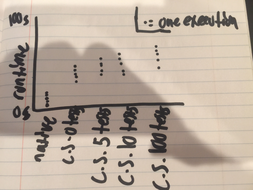
\includegraphics[scale=.75]{images/performance.png}}
%        \caption{\emph{This shows the run time difference between the
%native program and CrashSimulator in seconds.  Each dot indicates an
%        execution.  The X axis shows time values for native executions, and
%        executions under CrashSimulator with 0, 5, 10, and 100 tests
%        performed respectively.
%}}
%         \label{figure:performance}
%
%    \end{figure}

 \begin{table}[t]
    \scriptsize{}
    \begin{tabular}{l p{1cm} p{1cm} p{1.2cm} p{1cm}}
    \toprule{}
        Application     & Native Execution Time & Initial Recording Time & CrashSimulator Replay Time & rr Replay Time  \\
\hline
        {\tt wc}        & 0m0.007s              & 0m0.473s               & 0m0.668s                   & 0m0.112s        \\
        {\tt fmt}       & 0m0.007s              & 0m0.321s               & 0m0.707s                   & 0m0.111s        \\
        {\tt od}        & 0m0.036s              & 0m0.317s               & 0m0.689s                   & 0m0.101s        \\
        {\tt ptx}       & 0m0.008s              & 0m0.352s               & 0m0.769s                   & 0m0.087s        \\
        {\tt comm}      & 0m0.132s              & 0m0.371s               & 0m0.776s                   & 0m0.141s        \\
        {\tt pr}        & 0m0.135s              & 0m0.888s               & 0m1.017s                   & 0m0.141s        \\
    \bottomrule{}
    \end{tabular}
    \caption{This table contains the times required to execute several coreutils applications under different conditions.
             Native execution time is the time required to execute the application from the command line while
             CrashSimulator Replay time is the time required to execute it with the tool, using the null mutator with no checker configured.
             Initial recording time is the time required to create an initial recording with CrashSimulator.  rr replay time is the
             time required to replay an application using rr without CrashSimulator and is included to demonstrate the additional
             overhead added by CrashSimulator's other components.}
    \label{table:performance}
\end{table}


{\bf Findings.}
Overall, the performance running an application
under CrashSimulator is around
two orders of magnitude slower
than the original program executed without it.
As can be seen table~\ref{table:performance}, around 20\%
of this slow down is related to the additional overhead of {\tt rr}'s replay.
An additional portion is caused by the need to spin up Python's interpreter
before testing can begin.
In most cases
this slowdown is somewhat mitigated by CrashSimulator's ability to process
tests asynchronously. In other situations, it will be more efficient than
running the program natively, as {\tt rr's} replay does not require
actual execution of most system calls.  This means that CrashSimulator
avoids the system call overheads, such as I/O.
Even without these improvements, however, CrashSimulator's performance
cost is more
than manageable when the value it provides is taken into account.  The
cumulative runtime required to execute the tests required to produce the
results listed in Table~\ref{table:unexpectedtypes} is around 90 seconds.
Given this success, the increased time is worth the wait.
